% Blocks 1 + 2 of the HDC-RWKV expansion — token lookup + posiaqaation binding.
% Full-width standalone figure. Compile:  pdflatex arch_expand_input.tex

\documentclass[tikz,border=8pt]{standalone}
\usepackage{tikz}
\usepackage{amsmath,amssymb}
\usepackage{xcolor}
\usetikzlibrary{positioning,arrows.meta,calc,fit,backgrounds,decorations.pathreplacing}

\newcommand{\bV}{\mathbf{V}}
\newcommand{\bh}{\mathbf{h}}
\newcommand{\bipset}{\{-1,+1\}}

\definecolor{cBipolar}{HTML}{2C5282}
\definecolor{cBipolarLite}{HTML}{EBF4FF}
\definecolor{cCont}{HTML}{B7791F}
\definecolor{cPanelBg}{HTML}{FAFBFC}
\definecolor{cPanelBorder}{HTML}{CBD5E0}

\tikzset{
  block/.style={draw=cPanelBorder, fill=cPanelBg, thick, rounded corners=6pt,
                inner sep=8pt, minimum width=170mm},
  blockTitle/.style={font=\bfseries\normalsize, anchor=north west, inner sep=6pt},
  cellPos/.style={draw=cBipolar!50, fill=cBipolarLite, font=\small,
                  minimum width=9mm, minimum height=8mm, inner sep=0pt},
  cellNeg/.style={draw=cBipolar!50, fill=cBipolar!18, font=\small,
                  minimum width=9mm, minimum height=8mm, inner sep=0pt},
  idx/.style={font=\scriptsize\ttfamily, text=black!55},
  lbl/.style={font=\scriptsize\itshape, text=black!65, align=center},
  matlbl/.style={font=\scriptsize, text=cBipolar!85!black, align=center},
}

\begin{document}
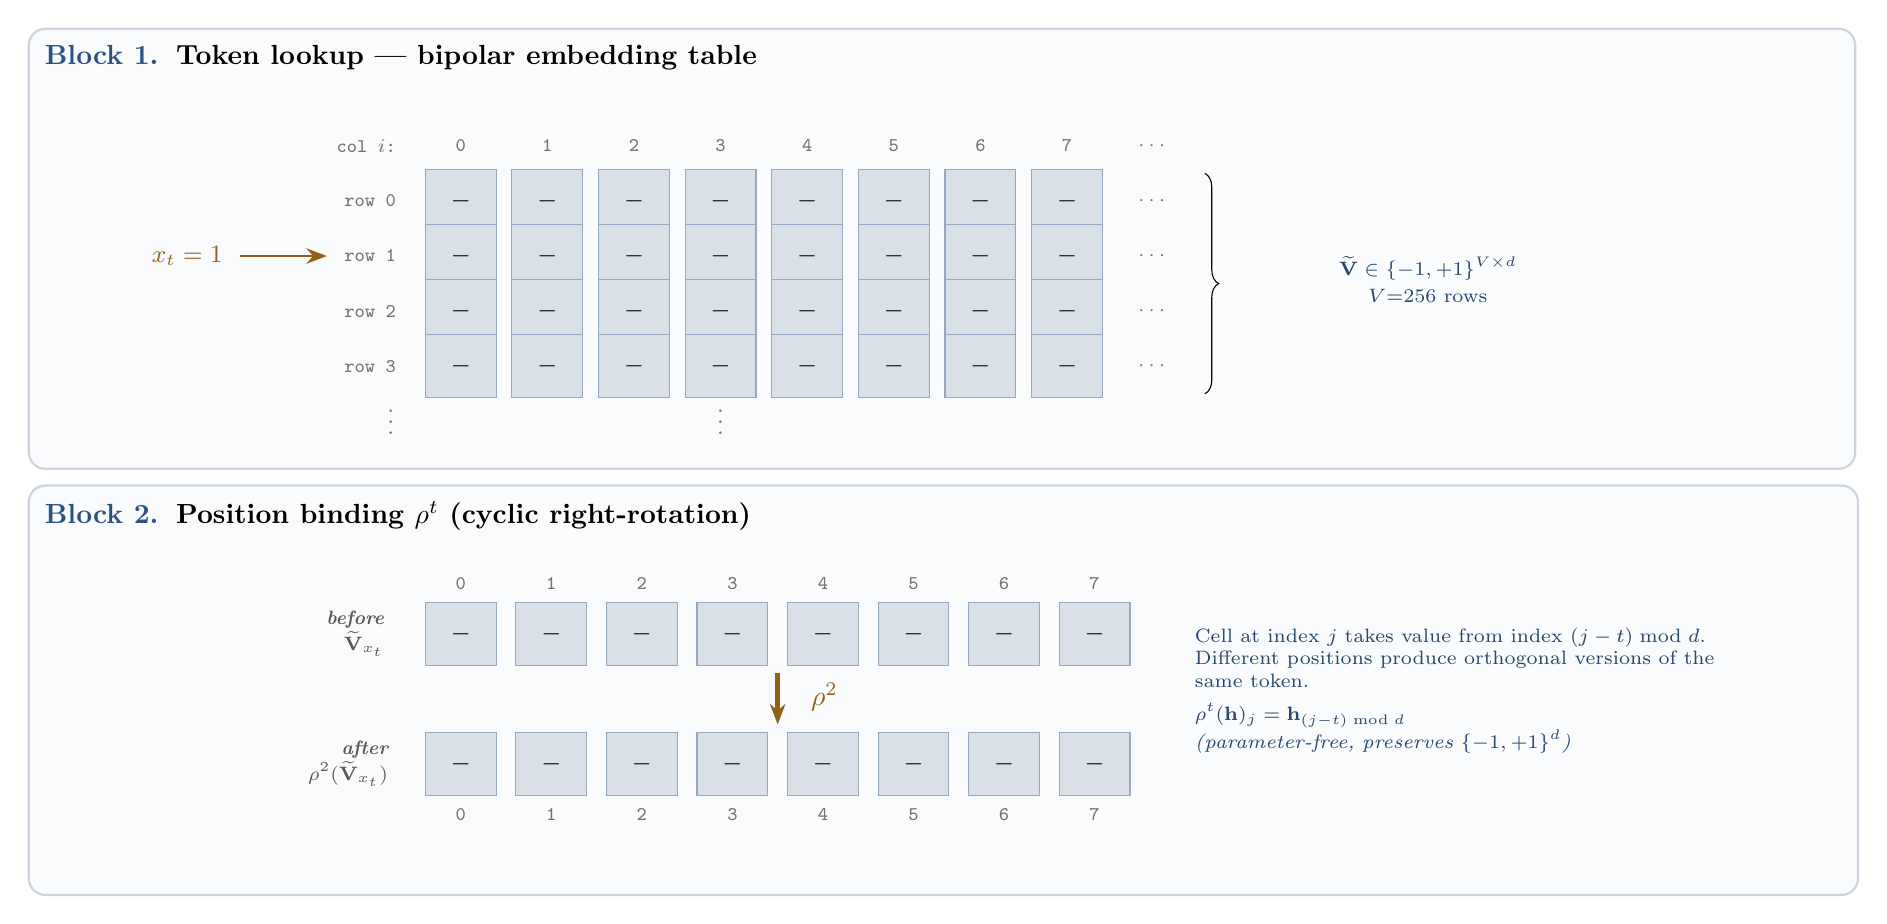
\begin{tikzpicture}

% ========== BLOCK 1: TOKEN LOOKUP ==========
\node[block, minimum height=159pt, anchor=north west, minimum width=660pt] (B1) at (0,0) {};
\node[blockTitle] at (B1.north west)
  {\textcolor{cBipolar}{Block 1.}\;\;Token lookup --- bipolar embedding table};

\begin{scope}[shift={(5.5,-1.5)}]
  \node[idx, anchor=east] at (-0.7, 0) {col $i$:};
  \foreach \j in {0,1,2,3,4,5,6,7}
    \node[idx] at (\j*1.1, 0) {\j};
  \node[idx] at (8*1.1, 0) {$\cdots$};

  \foreach \row/\y/\pat in {0/-0.7/{+,-,+,-,+,-,+,-},
                            1/-1.4/{-,+,-,+,-,+,-,+},
                            2/-2.1/{+,+,-,-,+,+,-,-},
                            3/-2.8/{+,-,-,+,+,+,-,-}} {
    \node[idx, anchor=east] at (-0.7, \y) {row \row};
    \foreach \v [count=\i from 0] in \pat {
      \ifx\v+
        \node[cellPos] (r\row_\i) at (\i*1.1, \y) {$+$};
      \else
        \node[cellNeg] (r\row_\i) at (\i*1.1, \y) {$-$};
      \fi
    }
    \node[idx] at (8*1.1, \y) {$\cdots$};
  }
  \node[idx, anchor=east] at (-0.7, -3.4) {$\vdots$};
  \node[idx] at (3*1.1, -3.4) {$\vdots$};

  \draw[decorate, decoration={brace, amplitude=5pt}]
    (8*1.1 + 0.65, -0.35) -- (8*1.1 + 0.65, -3.15);
  \node[matlbl, anchor=west] at (11.03, -1.7)
    {$\widetilde\bV \in \bipset^{V\times d}$\\[2pt] $V{=}256$ rows};

  \draw[-{Stealth[length=2.6mm]}, thick, cCont!80!black]
    (-2.8, -1.4) -- (-1.7, -1.4);
  \node[font=\small\bfseries, text=cCont!80!black, anchor=east]
    at (-2.9, -1.4) {$x_t = 1$};
\end{scope}

% ========== BLOCK 2: POSITION BINDING ==========
\node[block, minimum height=52mm, anchor=north west, minimum width=661pt] (B2) at (0,-58mm) {};
\node[blockTitle] at (B2.north west)
  {\textcolor{cBipolar}{Block 2.}\;\;Position binding $\rho^{t}$ (cyclic right-rotation)};

\begin{scope}[shift={(5.5,-7.7)}]
  \node[lbl, anchor=east, align=right] at (-0.85, 0)
     {\textbf{before}\\$\widetilde\bV_{x_t}$};
  \foreach \v [count=\i from 0] in {-,-,+,+,-,+,-,+} {
    \ifx\v+
      \node[cellPos] (in\i) at (\i*1.15, 0) {$+$};
    \else
      \node[cellNeg] (in\i) at (\i*1.15, 0) {$-$};
    \fi
    \node[idx, above=1pt of in\i] {\i};
  }

  \draw[-{Stealth[length=2.6mm]}, ultra thick, cCont!80!black]
    (3.5*1.15, -0.5) -- (3.5*1.15, -1.15);
  \node[font=\normalsize\bfseries, text=cCont!80!black, anchor=west]
    at (3.5*1.15 + 0.3, -0.8) {$\rho^{2}$};

  \node[lbl, anchor=east, align=right] at (-0.8, -1.65)
    {\textbf{after}\\$\rho^{2}(\widetilde\bV_{x_t})$};
  \foreach \v [count=\j from 0] in {-,+,-,-,+,+,-,+} {
    \ifx\v+
      \node[cellPos] (out\j) at (\j*1.15, -1.65) {$+$};
    \else
      \node[cellNeg] (out\j) at (\j*1.15, -1.65) {$-$};
    \fi
    \node[idx, below=1pt of out\j] {\j};
  }

  \node[matlbl, align=left, anchor=west, text width=68mm]
     at (9.2, -0.72)
    {Cell at index $j$ takes value from index $(j - t) \bmod d$.\\
     Different positions produce orthogonal versions of the same token.\\[4pt]
     $\rho^{t}(\bh)_j = \bh_{(j-t)\bmod d}$\\
     \emph{(parameter-free, preserves $\bipset^{d}$)}};
\end{scope}

\end{tikzpicture}
\end{document}
